\documentclass{article} 

\usepackage{geometry}
\usepackage{indentfirst}
\usepackage{fancyhdr}
\usepackage{caption}
\usepackage{graphicx}
\usepackage{enumitem}
\usepackage{hyperref}

\pagestyle{fancy}
\geometry{a4paper, margin=1in}
\captionsetup{labelformat=empty}
\graphicspath{ {../../assets/SDD_images/} }

\begin{document}

\title{Software Design Document for Viper Rocks!}
\author{Version 1.1.0}
\date{Group 2}

\maketitle
\tableofcontents
\newpage

\fancyhf{}
\fancyhead[C]{Software Design Document}
\fancyfoot[C]{\thepage}

\begin{table}[h!]
\centering
\caption{\textbf{Revision History}}
\begin{tabular}{|c|c|c|c|}
\hline
\textbf{Name} & \textbf{Date} & \textbf{Reasons for Changes} & \textbf{Version} \\
\hline
Tony Lau & 2/20/25 & First Draft & 1.0.0 \\
\hline
Tony Lau & 3/20/25 & Checkpoint 1; System Architecture and User Interface updated & 1.1.0 \\
\hline

\hline

\hline
\end{tabular}
\end{table}

\section{Introduction}
\subsection{Purpose}
This Software Design Specification Document (SDD) serves as a blueprint for developing the VIPER Rocks! citizen science application. It comprehensively details the core functionalities and architecture of the application, encompassing elements like the scouting, sizing, and classification tasks, user account creation, and database structure. This SDD equips the development team with the necessary guidance to construct a robust and well-organized system.
\subsection{Document Conventions}
This document uses bold for headings, bullet points for shorter information, and Times New Romans font at Size 12. Each higher-level requirement is to be inherited by the detailed requirement.
\subsection{Intended Audience and Reading Suggestions}
This Software Design Document caters to a diverse audience with varying technical background and interests. Here is a breakdown of the different types of readers and their primary concerns:
\begin{itemize}
	\item Software Developers: This document is for the people who want to understand and update the technical specifications and architecture of the software. It equips them to understand, maintain, and update the software’s core functionalities.
	\item Project Managers: This document allows them to understand how the software components interact to fulfill project requirements. It aids in planning development tasks, resource allocation, and overall project management.
	\item Users (Citizen Scientists): They will focus on the sections that explain how to utilize the VIPER Rocks! application effectively. This includes understanding its capabilities and limitations for contributing to scientific discovery.
	\item Testers: This document outlines the software’s requirements and design. Utilize this information to plan and execute comprehensive test cases, ensuring the application functions as intended.
\end{itemize}
 
\subsection{System Overview}
VIPER Rocks! is a web-based application designed for NASA’s Jet Propulsion Laboratory (JPL) that encourages citizen scientists with different backgrounds to contribute to the VIPER mission. By analyzing images captured by VIPER on its journey to the South Pole of the Moon, anyone can play a vital role in lunar exploration.

The application guides citizen scientists through a three-step process to analyze lunar rocks:
\begin{itemize}
	\item \textbf{Scouting:} Citizen scientists examine provided images to determine an approximate number of rocks. This allows the system to subdivide the original image into small sub-images.
	\item \textbf{Sizing:} Using the subdivided images from the scouting task, citizen scientists will utilize the sizing tool to trace and highlight various rocks in order to get their measurement. By analyzing rock size, scientists can map the lunar surface, determine rock size-frequency distributions (providing information on age, exposure history, and regolith maturity).
	\item \textbf{Classification:} Citizen scientists will be able to organize an individual rock’s shape into categories: angular, sub-angular, sub-rounded, and rounded. For more difficult rocks, there is an ambiguous category. Assessing shape information will allow scientists to have a better understanding on rock shape-frequency distributions.
\end{itemize}
As citizen scientists complete these tasks, their contributions are recorded in a central database.
This collective effort allows scientists to analyze vast amounts of data, ultimately leading to a
deeper understanding of the Moon’s geological makeup.

\section{System Architecture}
This section provides a high-level overview of the VIPER Rocks! application’s architecture and decomposes the system into its major modules/components.

\textbf{System Purpose and Goals}

The VIPER Rocks! system is a citizen science platform designed to engage the public in the research of lunar rocks. Here’s a breakdown of its key goals:
\begin{itemize}
	\item Crowdsourced Rock Scouting, Sizing, and Classification: Enable citizen scientists to participate in processing rock imagery provided by NASA’s VIPER mission, contributing valuable data for scientific analysis.
	\item Data Collection and Aggregation: Collect and aggregate results from citizen scientists to contribute to creating a comprehensive dataset for research purposes. 
\end{itemize}

\textbf{System Functionality Breakdown}

The VIPER Rocks! system can be viewed as a website-driven project offering the following core functionalities:
\begin{itemize}
	\item Secure User Access: Controls and regulates access to the website through a login and security system, ensuring authorized user participation.
	\item User Interface Management: Provide networked access to various user interface (UI) pages, allowing users to interact with the system for registration, login, task completion, and viewing results.
	\item Data Communication and Management: Manages data transfer (user information, rock images, task results, etc.) within a secure network environment.
	\item Citizen Science Workflow: Provides functionalities for a range of interface-specific tools citizen scientists use for scouting, sizing, and classification tasks.
	\item Administrator Workflow: Provides functionalities for a range of interface-specific tools users use with administrator roles for data analysis and management.
	\item Essential Utilities: Supports an assortment of powerful and essential utilities that contribute to the overall system operation, such as data storage, user management, and communication functionalities.
\end{itemize}
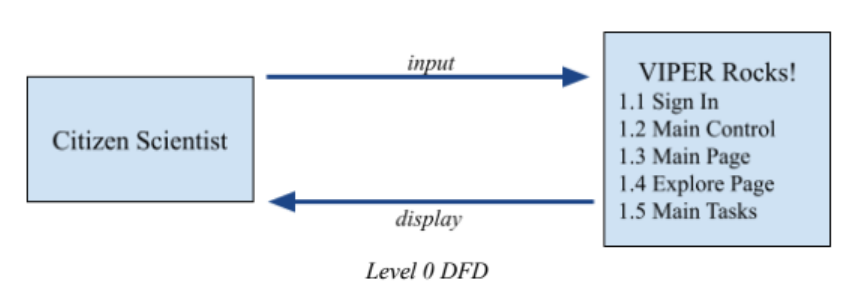
\includegraphics{DFD_0}

The system involves the citizen scientist user and the VIPER Rocks! application. The citizen scientist will give input and the system will return the corresponding module. \\
1.1 Sign In: User registration and login \\
1.2 Main Control: Connects and controls the different modules. \\
1.3 Main Page: The main landing page of the website. \\
1.4 Explore Page: The dashboard page that leads to the different rock image processing tasks. \\
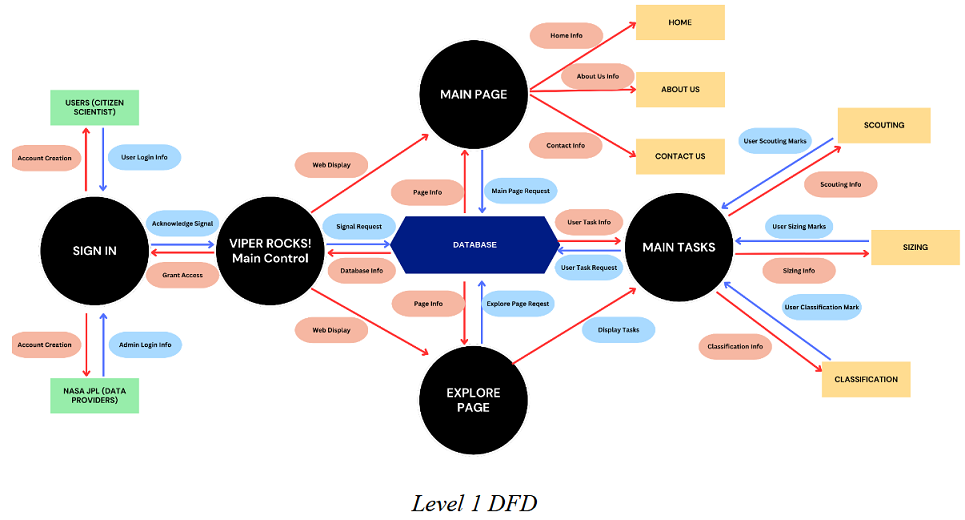
\includegraphics{DFD_1}

The VIPER Rocks! Data Flow Diagram (DFD) Level 1 highlights the major system components and their interactions. The DFD utilizes arrows to represent the flow of data, with red arrows signifying user-generated content and blue arrows indicating internal system data processing.

\textbf{System Components:}

The DFD is divided into several key areas, each represented by a circle:
\begin{itemize}
	\item 1.1 Sign-In manages user and administrator login functionalities.
	\item 1.2 VIPER Rocks! Main Control: The central processing unit that receives requests from various components and the database, coordinating responses throughout the system. 
	\item 1.3 Main Page: Serves as a central hub after successful login. It provides navigation options (“Home,” “About Us,” “Contact Us”), retrieves relevant information from the database for display, and interacts with the Main Control unit for further actions.
	\item 1.4 Explore Page: Allows users to browse and request different tasks. This page interacts with the database to retrieve information on available tasks for user participation.
\end{itemize}
There is also the database which is responsible for processing and storing all data requests and retrievals. It interacts with various components to manage data flow throughout the application.

\textbf{Data Flow:}
\begin{enumerate}
\item Users interact with the Sign In component, providing credentials.
	\begin{enumerate}[label=(\alph*)]
		\item Valid credentials grant access.
		\item Invalid credentials result in an error message.
	\end{enumerate}
\item The Main Control receives a request from the Sign-in component.
	\begin{enumerate}[label=(\alph*)]
		\item Upon successful login, the Main Control directs the user to the Main Page.
	\end{enumerate}
\item The Main Page retrieves information (e.g., navigation options, content) from the
database and displays it to the user.
\item Users can navigate from the Main Page to the Explore Page to view available tasks.
\item The Explore Page interacts with the database to retrieve task information and displays it
for user selection.
\item The Main Tasks component interacts with the database to store the user-contributed data.
\item Throughout the process, the Main Control unit receives requests from various components and facilitates communication with the database, ensuring smooth system operation.
\end{enumerate}
\section{User Interface}

\subsection{Overview of User Interface}
VIPER Rocks! follow Explorer 1: JPL’s Design System using React, Typescript, and TailwindCSS.

From the user’s perspective, VIPER Rocks! presents a seamless and user-friendly interface that facilitates an engaging and educational experience. The initial step involves creating an account where the users provide a strong password and store it securely with salting and hashing—emphasizing data collection for scientific purposes while ensuring privacy.

The home page welcomes users with an optional tutorial and showcases VIPER’s mission, purpose, and user feedback. JPL News Feed will be present for regular users from the science team, and contact information for bug reports or queries from JPL will add transparency—integration with OAuth, Facebook, Google login, Discord, and GitHub for optional log in.

The scouting page introduces the distribution of rocks within an image and a sizing task with intuitive desktop and mobile tools that enrich the scouting experience and lead to a separate menu for the classification task. The general design incorporates a side-daw navigation bar for tools, offering a unified experience across mobile and desktop platforms.

In summary, VIPER Rocks! aims to empower users to contribute meaningfully to scientific endeavors, providing a well-designed, educational, and rewarding platform while ensuring data security and accuracy—the detailed user manual supplements this overview, offering comprehensive guidance on system functionality.

\subsection{Screen Framework}
These can be mockups or actual screenshots of the various UI screens and popups. \\
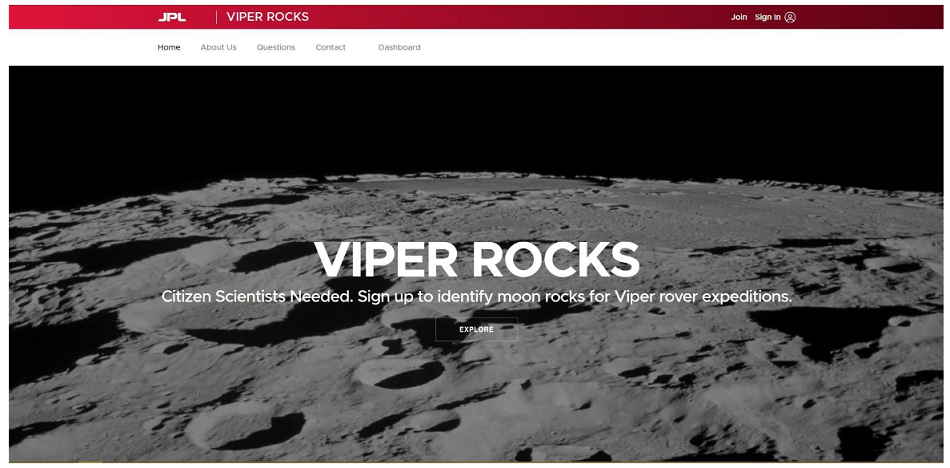
\includegraphics{home_page}
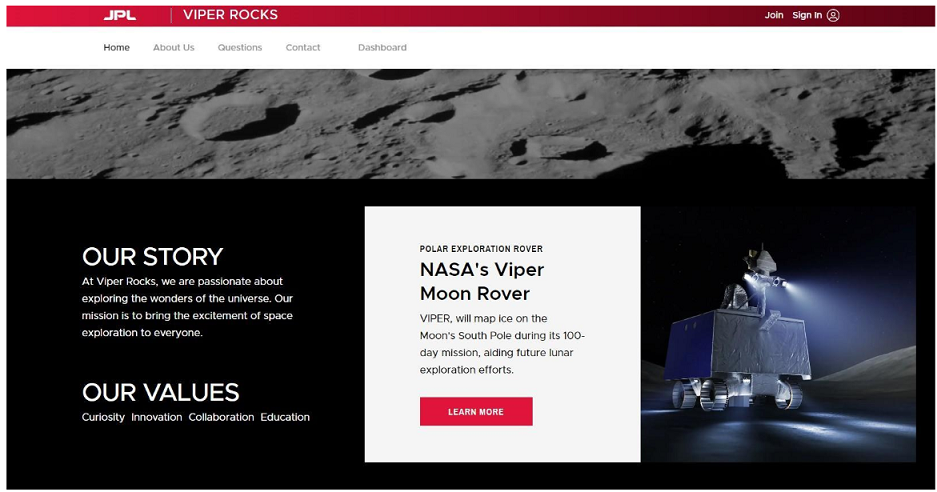
\includegraphics{home_page_2}
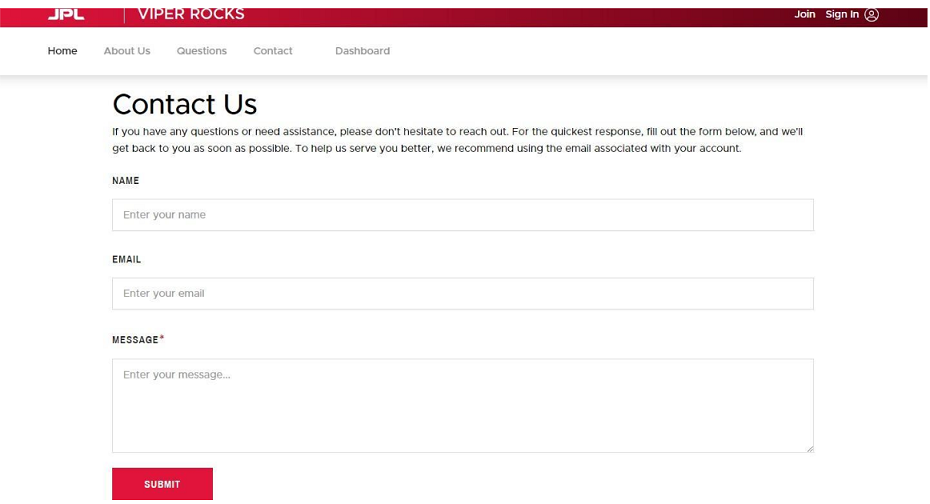
\includegraphics{contact_us_page}
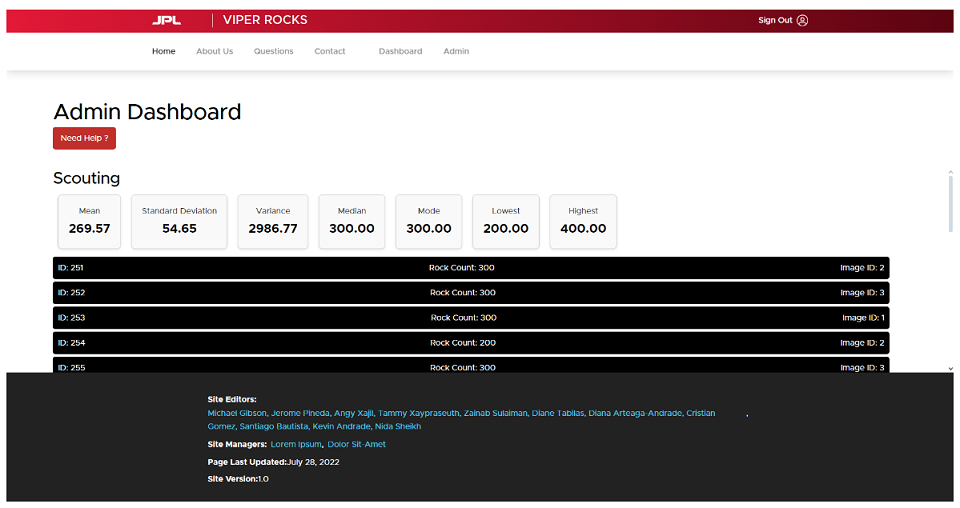
\includegraphics{admin_dashboard_page}
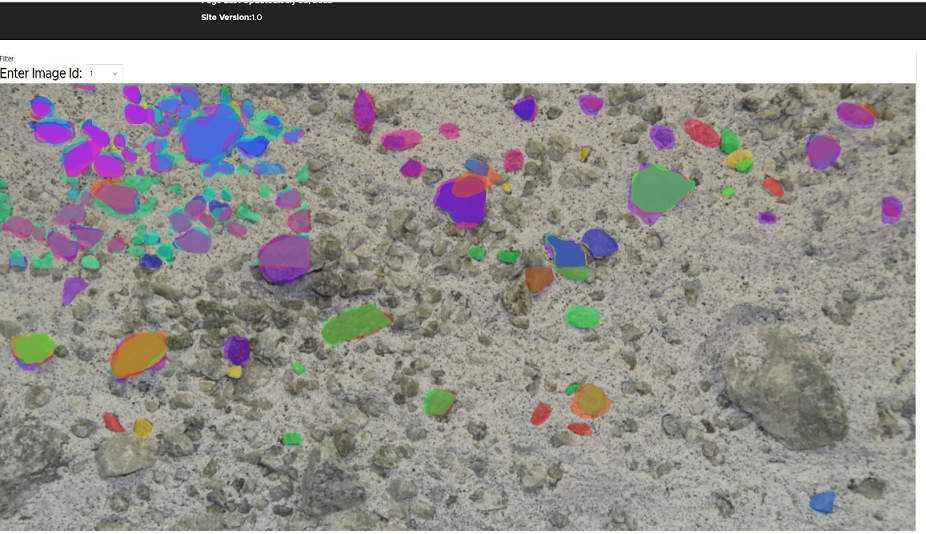
\includegraphics{scouting_page}
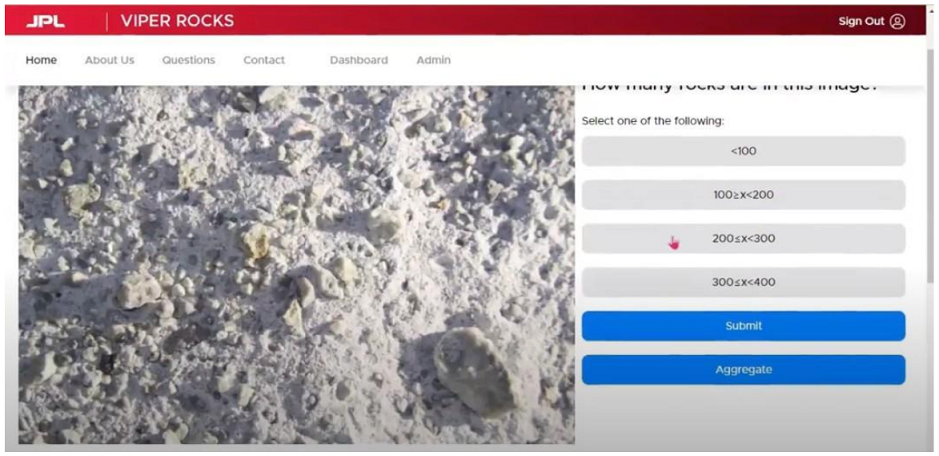
\includegraphics{scouting_page_2}
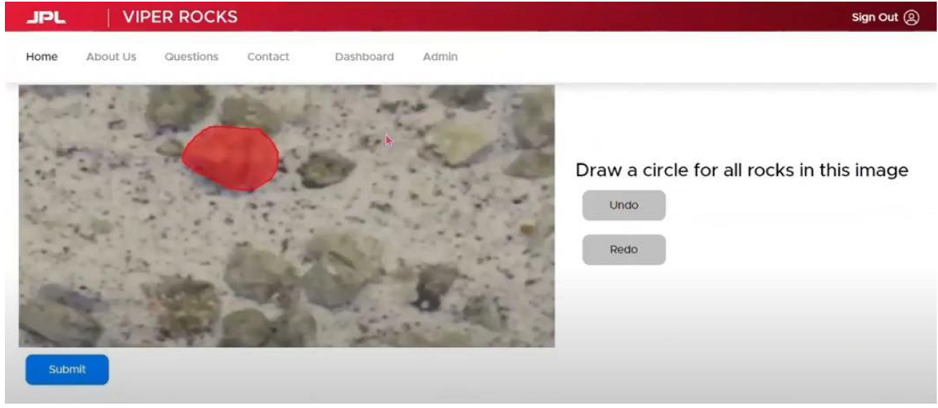
\includegraphics{sizing_page}
\section{Glossary}
\begin{itemize}
	\item NASA - National Aeronautics and Space Administration
	\item Selenology - Term for Lunar Geology
	\item SRS / SRD - Software Requirements Specification (Document)
	\item UI - User Interface
	\item VIPER - Volatiles Investigating Polar Exploration Rover
	\item Regolith - a region of loose unconsolidated rock and dust that sits atop a layer of bedrock
\end{itemize}

\section{References}
\begin{itemize}
	\item Software Design Document (SRS)
	\item Ascent Page: \href{https://ascent.cysun.org/project/project/view/227}{Link}
	\item \href{https://github.com/nasa-jpl/explorer-1}{Explorer-1: JPL's Design System}
\end{itemize}

\end{document}